\documentclass[a4paper]{article}
\usepackage[affil-it]{authblk}

\usepackage[UTF8]{ctex}
\usepackage{amsmath}
\usepackage{amssymb}
\usepackage{geometry}
\usepackage{graphicx}

\geometry{margin=1.5cm, vmargin={0pt,1cm}}
\setlength{\topmargin}{-1cm}
\setlength{\paperheight}{29.7cm}
\setlength{\textheight}{25.3cm}


\begin{document}
% =================================================
\title{Numerical Analysis homework \# 3}

\author{梁育玮 Liang Yuwei 3230102923
  \thanks{Electronic address: \texttt{liangyuwei631@gmail.com}}}
\affil{(Mathematics and Applied Mathematics 2302), Zhejiang University }
\date{\today}

\maketitle


% ============================================
\section*{I. Consider $s \in \mathbf{S}$ on [0,2]}
By computing, we can know that $s(1) = 1, s'(1)=-3, s''(1) = 6$

Assume $p(x) = ax^3 + bx^2+ cx + d$, then we have following:
\[\begin{cases}
    p(0) = d = 0, \\
    p(1) = a + b + c + d = 1, \\
    p'(1) = 3a + 2b + c = -3, \\
    p''(1) = 6a + 2b = 6
  \end{cases}
  \implies
  \begin{cases}
    a = 7, \\
    b = -18, \\
    c = 12, \\
    d = 0.
  \end{cases}
\]

So the cubic polynomial is $p(x) = 7x^3 - 18x^2 + 12x$. Since $s''(0) \neq 0$, $s(x)$ isn't a natural cubic spline.

\section*{II. Intepolating $f$ on [a,b]}
\subsection*{II-a}
By theorem 3.14, The set of splines $\mathbb{S}^1_2(x_1,x_2,\cdots,x_n)$ is a linear space with dimension $n+1$, but only $n$ conditions are given, so an addition condition is needed to determine the spline uniquely.

\subsection*{II-b}
The table of divided differences is as follows:
\[
\begin{array}{c|ccc}
  x_i & f_i &  &  \\
  x_i & f_i & m_i &  \\
  x_{i+1} & f_{i+1} & \dfrac{f_{i+1}-f_i}{x_{i+1}-x{i}} &  \dfrac{f_{i+1}-f{i}-m_i(x_{i+1}-x_i)}{(x_{i+1}-x_i)^2}\\
\end{array}
\]

Then the Newton formula yeilds:
\[
  p_i(x) = f_i + m_i(x-x_i) + \dfrac{f_{i+1}-f{i}-m_i(x_{i+1}-x_i)}{(x_{i+1}-x_i)^2}(x-x_i)^2
\] 

\subsection*{II-c}
Denote $k_i = \dfrac{f_{i+1}-f_i}{x_{i+1}-x{i}}$, then we have $p_i'(x_i+1) = 2k_i - m_i$.$s \in \mathcal{C}^1$ implies $p_i'(x_{i+1}) = p_{i+1}'(x_{i+1})$ , i.e. \[
2k_i - m_i = m_{i+1} .
\]

Then we can compute $m_i$ sequentially

\section*{III. Let $s_1(x) = 1 + c(x+1)^3$}
By computing, we can know that $s_1(0) = 1 + c , s_1'(0) = 3c, s_1''(0) = 6c$. Assume $s_2(x) = a x^3 +b x^2 + dx + e$, The we have following:
\[\begin{cases}
    s_2(0) = e = 1 + c, \\
    s_2'(0) = d = 3c, \\
    s_2''(0) = 2b = 6c \\
    s_2''(1) = 6a + 2b = 0 
  \end{cases}
  \implies
  \begin{cases}
    a = -c, \\
    b = 3c, \\
    d = 3c, \\
    e = 1 + c.
  \end{cases}
\]

So $s_2(x) = -cx^3 + 3cx^2 + 3cx + 1 + c$. 

Let $s(1) = 0$, then $6c + 1 = -1$, thus $c = -\dfrac{1}{3}$.
\section*{IV. Consider $f(x) = \cos(\frac{\pi}{2}x)$}
\subsection*{IV-a}
We have $f(-1) = 0, f(0) = 1, f(1) = 0$, set
\[
s=\begin{cases}
  s_1(x) = a_1x^3 + b_1 x^2 + c_1 x + 1, & x \in [-1,0], \\
  s_2(x) =  a_2x^3 + b_2 x^2 + c_2 x + 1& x \in [0,1].
\end{cases}
\] 
Then we have, 
\[\begin{cases}
  s_1(-1) = -a_1 + b_1 - c_1 + 1 =0, \\
  s_1''(0) = -6 a_1  +2 b_1 = 0, \\
  s_2(1) = a_2 + b_2 + c_2 + 1 = 0\\
  s_2''(1) = 6 a_2 + 2 b_2 = 0,\\
  c_1 = c_2 ,\\
  b_1 = b_2.
\end{cases}
\implies
\begin{cases}
  a_1 = -\dfrac{1}{2}, \\
  b_1 = -\dfrac{3}{2}, \\
  c_1 = 0, \\
  a_2 = \dfrac{1}{2}, \\
  b_2 = -\dfrac{3}{2}, \\
  c_2 = 0.
\end{cases}
\]
Thus the cubic spline is
\[
s(x) = \begin{cases}
  -\dfrac{1}{2}x^3 - \dfrac{3}{2} x^2 + 1, & x \in [-1,0], \\
  \dfrac{1}{2}x^3 - \dfrac{3}{2} x^2 + 1, & x \in [0,1].
\end{cases}
\]

\subsection*{IV-b}
The intergal of $[s''(x)]^2$ is

\begin{align*}
  \int_{-1}^{1} [s''(x)]^2dx &= \int_{-1}^{0} [s_1''(x)]^2dx + \int_{0}^{1} [s_2''(x)]^2dx \\
  &= \int_{-1}^{0} (-3x -3)^2dx + \int_{0}^{1} (3x-3)^2dx \\
  &= 3 + 3 = 6 .
\end{align*}

(i) Let $g(x)$ be the quadratic polynomial that interpolates $f$ at -1, 0, 1, then $g(x) = -x^2 +1$. The error is $f(x) - g(x) = \cos(\dfrac{\pi}{2}x) - \dfrac{1}{2}x^2 + \dfrac{1}{2}$, and the intergal for $g(x)$ is

\begin{align*}
  \int_{-1}^{1} [g''(x)]^2dx &= \int_{-1}^{1} 4dx = 8 > 6  .
\end{align*}

(ii) Let $g(x)$ be $f(x)$ itself, then the intergal is 

\begin{align*}
  \int_{-1}^{1} [f''(x)]^2dx &= \int_{-1}^{1} \dfrac{\pi^4}{16} \cos^2(\dfrac{\pi}{2}x)dx = \dfrac{\pi^4}{16} \int_{-1}^{1} \dfrac{1+\cos(\pi x)}{2}dx = \dfrac{\pi^4}{16} \approx 6.0757 > 6.
\end{align*}

So the theorem holds for thses two cases.

\section*{V. the quadratic B-spline $B_i^2(x)$}
\subsection*{V-a}
By definition, we have
\begin{align*}
  B_i^2(x) &= \dfrac{x-t_{i-1}}{t_{i+1} - t_{i-1}}\hat{B}_i(x) + \dfrac{t_{i+2} - x}{t_{i+2} - t_i}\hat{B}_{i+1}(x)\\
  &= \begin{cases}
    \frac{(x-t_{i-1})^2}{(t_{i+1} - t_{i-1})(t_i - t_{i-1})}, & x \in [t_{i-1}, t_i], \\
    \frac{(x-t_{i-1})(t_{i+1} - x)}{(t_{i+1}- t_i)(t_{i+1}-t_{i-1})} + \frac{(t_{i+2} - x)(x-t_i)}{(t_{i+2}-t_i)(t_{i+1} - t_i)}, & x \in [t_i, t_{i+1}], \\
    \frac{(t_{i+2}-x)^2}{(t_{i+2}-t_{i})(t_{i+2}-t_{i+1})}, & x \in [t_{i+1}, t_{i+2}], \\
    0, & \text{otherwise}.
  \end{cases}
\end{align*}

\subsection*{V-b}
The derivative of $B_i^2(x)$ is
\[
  \frac{\text{d}}{\text{d}x}B_i^2(x)= \begin{cases}
    \frac{2(x-t_{i-1})}{(t_{i+1} - t_{i-1})(t_i - t_{i-1})}, & x \in [t_{i-1}, t_i], \\
    \frac{t_{i+1} + t_{i-1} -2x}{(t_{i+1}- t_i)(t_{i+1}-t_{i-1})} + \frac{t_{i} + t_{i+2}  -2 x}{(t_{i+2}-t_i)(t_{i+1} - t_i)}, & x \in [t_i, t_{i+1}], \\
    \frac{-2(t_{i+2}-x)}{(t_{i+2}-t_{i})(t_{i+2}-t_{i+1})}, & x \in [t_{i+1}, t_{i+2}], \\
    0, & \text{otherwise}.
  \end{cases}
\]

Substituting $x = t_i$ into the first equation, we get:
\[
\left. \frac{\text{d}}{\text{d}x} B_i^2(x) \right|_{x=t_i} = \frac{2}{t_{i+1} - t_{i-1}}.
\]

And substituting $x = t_{i}$ into the second equation, we get:
\begin{align*}
  \left. \frac{\text{d}}{\text{d}x} B_i^2(x) \right|_{x=t_i} &=     \frac{t_{i+1} + t_{i-1} -2t_i}{(t_{i+1}- t_i)(t_{i+1}-t_{i-1})} + \frac{t_{i+2}  - t_i}{(t_{i+2}-t_i)(t_{i+1} - t_i)} \\
  &= \frac{2}{t_{i+1} - t_{i-1}}-\frac{1}{t_{i+1} - t_i} + \frac{1}{t_{i+1} - t_i}\\
  &= \frac{2}{t_{i+1} - t_{i-1}}.
\end{align*}
Thus $\frac{\text{d}}{\text{d}x}B_i^2(x)$ is continuous at $t_i$.
Similarly, we can verify that the $\frac{\text{d}}{\text{d}x}B_i^2(x)$ is continuous at $t_{i+1}$ by computing 
\[
\left. \frac{\text{d}}{\text{d}x} B_i^2(x) \right|_{x=t_{i+1}} = \frac{-2}{t_{i+2} - t_{i+1}}.
\]

\subsection*{V-c}
It's easy to see that when $x \in (t_{i-1,t_i}], \dfrac{\text{d}}{\text{d}x} B_i^2(x) > 0$ and when $x \in [t_{i+1},t_{i+2}), \dfrac{\text{d}}{\text{d}x} B_i^2(x) < 0$. Thus $x*$ only can be in $(t_{i},t_{i+1})$.

Let $\left. \frac{\text{d}}{\text{d}x} B_i^2 \right|_{x=x*} = 0$, then we have

Then we have 
\begin{align*}
    &\frac{t_{i+1} + t_{i-1} -2x^*}{(t_{i+1}- t_i)(t_{i+1}-t_{i-1})} + \frac{t_{i} + t_{i+2}  -2 x^*}{(t_{i+2}-t_i)(t_{i+1} - t_i)}  = 0\\
    &\implies x^* = \frac{t_{i+1} t_{i+2} + t_{i-1} t_{i+2} - t_{i+1} t_i - t_{i-1} t_i}{t_{i+2} - t_i - t_{i+1} + t_{i-1}}.    .
\end{align*}

\subsection*{V-d}
It's easy to see that $B_i^2(x) \geq 0$ for all $x$. And by Corollary 3.38, we have 
$$\sum_{i=-\infty}^{\infty} B_i^2(x) = 1, \quad\forall  x\in \mathbb{R}$$
Since for all $x$, there must be two $B_i^2(x)$ that are not zero, we have $B_i^2(x)<1$.

\subsection*{V-e}
Using the result of V-a, we can plot the graph of $B_i^2(x)$ as follows (Figure \ref{fig:1}), \textit{the figure is colourful and may not be clear in black and white}.
\begin{figure}[h]
  \centering
  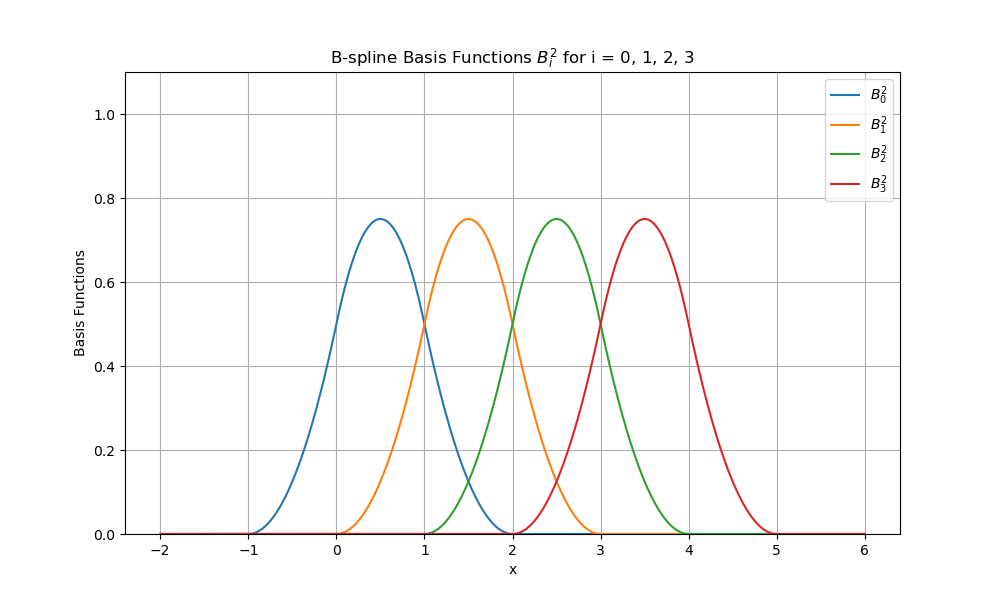
\includegraphics[width=0.5\textwidth]{B-spline.png}
  \caption{The graph of $B_i^2(x)$}
  \label{fig:1}
\end{figure}

\section*{VI. Verify Theorem 3.32 algebraically for the case of $n = 2$} 
To make the notation clear, we denote $[t_{i-1}, t_i, t_{i+1},t_{i+2}](t-x)^2_+$ as $(t-x)^2_+{[t_{i-1}, t_i, t_{i+1},t_{i+2}]}$, which fit the notation in the Chapter 2. And we donote $s(x) = (t_{i+2}-t_i)(t-x)^2_+[t_{i-1},t_i,t_{i+1},t_{i+2}]$.

Since $(t_j -t_{i+1})_+^2 = 0$ for $j = i-1, i, i+1$, we can easily compute that \[s(t_{i+1}) = \frac{(t_{i+2}-t_{i+1})^2}{(t_{i+2}-t_{i})(t_{i+2}-t_{i+1})} = B^2_i(t_{i+1})\]

And we have
\begin{align*}
  s(t_{i}) &= (t-t_{i+1})^2_+{[t_{i-1}, t_i, t_{i+1},t_{i+2}]}\\
  &= (t-t_{i})^2{[t_{i-1}, t_i, t_{i+1},t_{i+2}]} - (t_{i}-t)^2_+{[t_{i-1}, t_i, t_{i+1},t_{i+2}]}\\
&= - (t_{i}-t)^2_+{[t_{i-1}, t_i, t_{i+1},t_{i+2}]}\\
&=\frac{(t_i-t_{i-1})^2}{(t_{i+1} - t_{i-1})(t_i - t_{i-1})}\\
&= B^2_i(t_{i}).
\end{align*}
where the second equality is due to the fact that $(f + g)[x_i,\cdots,x_{i+n}] = f[x_i,\cdots,x_{i+n}] + g[x_i,\cdots,x_{i+n}]$ and $(t - x)^2_+ +(x-t)^2_+ = (x-t)^2$; the third from the fact that $(t-x)^2{[t_{i-1}, t_i, t_{i+1},t_{i+2}]} = 0$; and the forth can be computed similarly to $s(t_{i+1})$.

And we have $s(x)  = 0$ for all $x \notin [t_{i-1},t_{i+2}]$, and since $(t - x)_+^2 \in \mathcal{C}^1$, we have $s(x) \in \mathcal{C}^1$. And by the definition, we can know $\left. s(x)\right|_{[t_j,t_j+1]}$ is a quadratic polynomial. So $s(x) \in \mathbb{S}^1_2$.

And we have $s'(t_{i}) =\left. \frac{\text{d}}{\text{d}x} B_i^2\right|_{x=t_{i}} = 0 $, and $s(t_j) = B^2_i(t_j)$ for $j = i-1, i, i+1 \text{ and } i+2$. Since the dimension of $\mathbb{S}_2^1$ is $n+1$, $n+1$ conditions can determine the quadratic spline uniquely. Thus $s(x) = B^2_i(x)$.

\textbf{remark:} \textit{the proof may be a little long, primarily because the assigment requires to verify the theorem "algebraically"}
\section*{VII. Scaled integral of B-spline}
By the Theorem on derivative of B-spline, we have
\[
\frac{\text{d}}{\text{d}x} B_i^n(x) = \frac{n}{t_{i+n-1} - t_{i-1}}B_{i}^{n-1}(x) - \frac{n}{t_{i+n} - t_{i}}B_{i+1}^{n-1}(x).
\]

Integrating both sides of the above equation from $t_{i-1}$ to $t_{i+n}$, we get
\begin{align*}
  B_i^{n}(t_{i+n}) - B_i^{n}(t_{i-1})  & =  \int_{t_{i-1}}^{t_{i+n}} \frac{n}{t_{i+n-1} - t_{i-1}}B_{i}^{n-1}(x) - \frac{n}{t_{i+n} - t_{i}}B_{i+1}^{n-1}(x)dx\\  
          & = \frac{n}{t_{i+n-1}-t_{i-1}}\int_{t_{i-1}}^{t_{i+n-1}} B_{i}^{n-1}(x)dx - \frac{n}{t_{i+n} - t_{i}}\int_{t_{i}}^{t_{i+n}} B_{i+1}^{n-1}(x)dx\\
\end{align*}


Since $B_i^{n}(t_{i+n}) = B_i^{n}(t_{i-1}) = 0$, we have

\[
 \frac{1}{t_{i+n-1}-t_{i-1}}\int_{t_{i-1}}^{t_{i+n-1}} B_{i}^{n-1}(x)dx = \frac{1}{t_{i+n} - t_{i}}\int_{t_{i}}^{t_{i+n}} B_{i+1}^{n-1}(x)dx\\
\]

Then we can conclude that the scaled integral of B-spline over its support is independent of its index $i$ by induction.

\section*{VIII. Symmetric Polynomials}
\subsection*{VIII-a}
Without loss of generality, we can assume $i = 1$

(1) when $m =  2$, the table of divided differences is as follows:
\[\begin{array}{c|ccc}
  x_1 & x_1^2 &  \\
  x_2 & x_2^2 & x_1+x_2 &  \\
  x_3 & x_3^2 & x_2+x_3 &  1\\
\end{array}\]
where the value of dialog are the $x^2[x_1]$, $x^2[x_1,x_2]$ and $x^2[x_1,x_2,x_3]$ respectively.

We have $\tau_2(x_1) = x^2_1$, $\tau_1(x_1,x_2) = x_1 + x_2$ and $\tau_3(x_1,x_2,x_3) = 1$. Thus the Theorem holds for $m$ = 2. 

(2) when $m = 4$, the table of divided differences is as follows:
\[
\begin{array}{c|ccccc}
  x_1 & x_1^4 &  &  &  & \\
  x_2 & x_2^4 & (x_1 + x_2)(x_1^2 + x_2^2) &  &  & \\
  x_3 & x_3^4 & (x_2 + x_3)(x_2^2 + x_3^2) & x_1^2 + x_2^2 + x_3^2 + x_1 x_2 + x_2 x_3 + x_3 x_1 &  & \\
  x_4 & x_4^4 & (x_3 + x_4)(x_3^2 + x_4^2) & x_2^2 + x_3^2 + x_4^2 + x_2 x_3 + x_2 x_4 + x_3 x_4 & x_1 + x_2 + x_3 + x_4 & \\
  x_5 & x_5^4 & (x_4 + x_5)(x_4^2 + x_5^2) & x_3^2 + x_4^2 + x_5^2 + x_3 x_4 + x_3 x_5 + x_4 x_5 & x_2 + x_3 + x_4 + x_5 & 1 \\
\end{array}
\]

And we can rewrite the table as follows:
\[
\begin{array}{c|ccccc}
  x_1 & x_1^4 &  &  &  & \\
  x_2 & x_2^4 & \tau_3(x_1, x_2) &  &  & \\
  x_3 & x_3^4 & \tau_3(x_2, x_3) & \tau_2(x_1, x_2, x_3) &  & \\
  x_4 & x_4^4 & \tau_3(x_3, x_4) & \tau_2(x_2, x_3, x_4) & \tau_1(x_1, x_2, x_3, x_4) & \\
  x_5 & x_5^4 & \tau_3(x_4, x_5) & \tau_2(x_3, x_4, x_5) & \tau_1(x_2, x_3, x_4, x_5) & \tau_0(x_1, x_2, x_3, x_4, x_5) \\
\end{array}
\]
from the above table, we can see that the Theorem holds for $m = 4$.

\section*{VIII-b}
Let's first prove a lemma that for any $k,i \text{ and } n$, We have
By the lemma on the recursive relation on complete symmetric polynomials, we have 
\begin{align*}
  \tau_k(x_1, x_2, \cdots, x_{n+1}) &= \tau_k(x_1, x_2, \cdots, x_{n}) + x_{i+n}\tau_{k-1}(x_1, x_2, \cdots, x_{n+1})\\
  & = \tau_k(x_2, x_3, \cdots, x_{n+1}) + x_1\tau_{k-1}(x_1, x_2, \cdots, x_{n+1}).\\
\end{align*}
Thus, 
\[
\dfrac{ \tau_k(x_{2}, x_{3}, \cdots, x_{n+1})-\tau_k(x_1, x_2, \cdots, x_n) }{x_{n+1} - x_1} = \tau_{k-1}(x_1, x_{2}, \cdots, x_{n+1})
\]

Using above lemma, we can write the table of divided differences as follows:
\[
\begin{array}{c|cccccc}
  \tau_n(x_1) & x_1^n &  &  &  &  \\
  \tau_n(x_2) & x_2^n & \tau_{n-1}(x_1, x_2) &  &  &  \\
  \tau_n(x_3) & x_3^n & \tau_{n-1}(x_2, x_3) & \tau_{n-2}(x_1, x_2, x_3) &  &  \\
  \tau_n(x_4) & x_4^n & \tau_{n-1}(x_3, x_4) & \tau_{n-2}(x_2, x_3, x_4) & \tau_{n-3}(x_1, x_2, x_3, x_4) &  \\
  \tau_n(x_5) & x_5^n & \tau_{n-1}(x_4, x_5) & \tau_{n-2}(x_3, x_4, x_5) & \tau_{n-3}(x_2, x_3, x_4, x_5) & \tau_{n-4}(x_1, x_2, x_3, x_4, x_5) \\
  \vdots & \vdots & \vdots & \vdots & \vdots & \ddots \\
  \tau_n(x_n) & x_n^n & \tau_{n-1}(x_{n-1}, x_n) & \tau_{n-2}(x_{n-2}, x_{n-1}, x_n) & \cdots &\cdots& \tau_{0}(x_1, x_2, \ldots, x_n) \\
\end{array}
\]

Similarly, the value of the dialog is divided differences respectively. Thus the Theorem holds for any $n$.
% ===============================================
\end{document}
